% The encodings of the stored numbers: what each represents of one element's values.  One component
% of the tangent over the element's points (dots) on the codec's grid of representable values; sigma
% is the element's largest stored magnitude.  Below each panel, the bits of a code.
\documentclass[border=2pt]{standalone}
% Shared preamble of the format diagrams: colours of the paper's figures (paper_figures.py) and
% the drawing styles.  Each diagram is a standalone document built to a PDF of the text width.
\usepackage{amsmath,amssymb}
\usepackage{tikz}
\usetikzlibrary{arrows.meta,calc,decorations.pathreplacing,patterns,positioning}

\definecolor{cindex}{HTML}{BDBDBD}  % column indices, offsets, row pointers
\definecolor{cvalue}{HTML}{6E6E6E}  % floating-point values (BSR)
\definecolor{cpoint}{HTML}{1B9E77}  % quadrature-point store
\definecolor{celem}{HTML}{1F78B4}   % element matrix
\definecolor{cqbsr}{HTML}{A6761D}   % quantized BSR
\definecolor{cscale}{HTML}{E6AB02}  % scales
\definecolor{cmean}{HTML}{7570B3}   % f32 element mean

\tikzset{
  >={Stealth[length=4pt]},
  grid/.style={draw=black!45, line width=0.25pt},
  frame/.style={draw=black!70, line width=0.5pt},
  title/.style={font=\small\bfseries, anchor=west, inner sep=0pt},
  lab/.style={font=\footnotesize, inner sep=1pt},
  note/.style={font=\scriptsize, text=black!75, inner sep=1pt, execute at begin node={\hyphenpenalty=10000\exhyphenpenalty=10000}},
  num/.style={font=\tiny, inner sep=0pt},
  brace/.style={decorate, decoration={brace, amplitude=3pt, raise=1pt}, line width=0.4pt},
  arr/.style={->, line width=0.5pt, black!70},
  pad/.style={pattern=north east lines, pattern color=black!30},
}

% \cell{x}{y}{w}{h}{fill}: a filled rectangle with a thin outline, lower-left corner at (x,y).
\newcommand{\cell}[5]{\filldraw[fill=#5, grid] (#1,#2) rectangle ++(#3,#4);}
% \blk{x}{y}{s}{fill}: a 3x3 block of side s with its 3x3 entry grid.
\newcommand{\blk}[4]{%
  \filldraw[fill=#4, grid] (#1,#2) rectangle ++(#3,#3);
  \draw[draw=white, line width=0.25pt] (#1,#2) ++(#3/3,0) -- ++(0,#3) ++(#3/3,0) -- ++(0,-#3);
  \draw[draw=white, line width=0.25pt] (#1,#2) ++(0,#3/3) -- ++(#3,0) ++(0,#3/3) -- ++(-#3,0);
  \draw[grid] (#1,#2) rectangle ++(#3,#3);}
% \vthree{x}{y}{fill}: a 3-vector (one node's components) as three small cells, left end at (x,y).
\newcommand{\vthree}[3]{\foreach \k in {0,1,2} \filldraw[fill=#3, grid] (#1+\k*0.14,#2) rectangle ++(0.14,0.14);}
% \op{x}{y}{symbol}: an operation in a small circle.
\newcommand{\op}[3]{\node[circle, draw=black!70, line width=0.4pt, inner sep=0.5pt, minimum size=9pt, font=\tiny] at (#1,#2) {#3};}

\usetikzlibrary{shapes.geometric}
\begin{document}
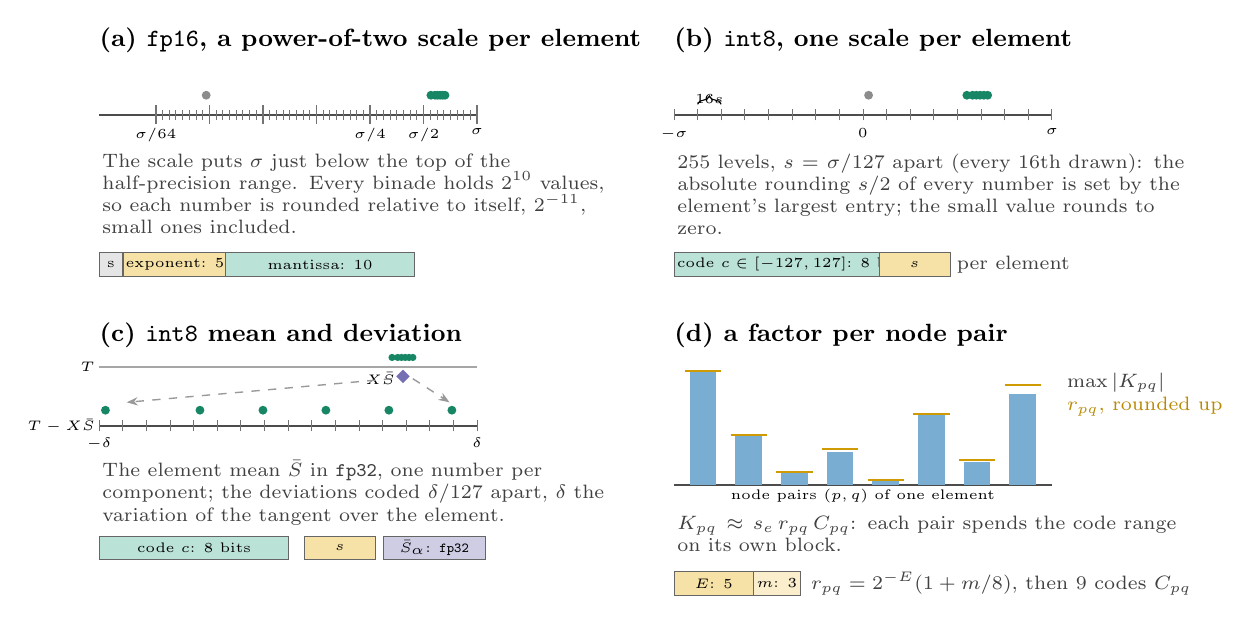
\begin{tikzpicture}
  \tikzset{
    axis/.style={draw=black!70, line width=0.5pt},
    tick/.style={draw=black!55, line width=0.3pt},
    val/.style={circle, fill=cpoint!85!black, inner sep=0pt, minimum size=3.2pt},
    bits/.style={draw=black!60, line width=0.3pt, font=\tiny, minimum height=0.3cm, inner sep=1pt},
    expl/.style={note, anchor=north west, align=left, text width=6.6cm},
  }
  \def\W{4.8}
  % one component over the element's points, in units of sigma: a cluster near 0.6 (and, in (a)
  % and (b), one small value of another component)
  \def\vals{0.55, 0.58, 0.6, 0.62, 0.64, 0.66}

  % ---------------------------------------------------------------- (a) fp16, scaled
  \begin{scope}[shift={(0,3.75)}]
    \node[title] at (0, 3.15) {(a) \texttt{fp16}, a power-of-two scale per element};
    \draw[axis] (0,2.2) -- (\W,2.2);
    \foreach \k in {0,...,6} {
      \pgfmathsetmacro{\x}{\W-0.68*\k}
      \draw[tick, line width=0.5pt] (\x,2.08) -- (\x,2.32);
      \ifnum\k<6 \foreach \j in {1,...,7} \draw[tick] ({\x-0.68+0.68*\j/8},2.14) -- ++(0,0.12); \fi
    }
    \node[num, anchor=north] at (\W,2.04) {$\sigma$};
    \node[num, anchor=north] at (\W-0.68,2.04) {$\sigma/2$};
    \node[num, anchor=north] at (\W-1.36,2.04) {$\sigma/4$};
    \node[num, anchor=north] at (\W-4.08,2.04) {$\sigma/64$};
    \foreach \v in \vals \node[val] at ({\W+0.68*ln(\v)/ln(2)}, 2.45) {};
    \node[val, fill=black!45] at ({\W+0.68*ln(0.03)/ln(2)}, 2.45) {};
    \node[expl] at (0,1.75) {The scale puts $\sigma$ just below the top of the half-precision range.
      Every binade holds $2^{10}$ values, so each number is rounded relative to itself, $2^{-11}$, small
      ones included.};
    \node[bits, minimum width=0.3cm, fill=black!10] at (0.15,0.3) {s};
    \node[bits, minimum width=1.3cm, fill=cscale!35, anchor=west] at (0.3,0.3) {exponent: 5};
    \node[bits, minimum width=2.4cm, fill=cpoint!30, anchor=west] at (1.6,0.3) {mantissa: 10};
  \end{scope}

  % ---------------------------------------------------------------- (b) int8, one scale per element
  \begin{scope}[shift={(7.3,3.75)}]
    \node[title] at (0, 3.15) {(b) \texttt{int8}, one scale per element};
    \draw[axis] (0,2.2) -- (\W,2.2);
    \foreach \j in {0,...,16} \draw[tick] ({\W*\j/16},2.13) -- ++(0,0.14);
    \node[num, anchor=north] at (0,2.04) {$-\sigma$};
    \node[num, anchor=north] at (\W/2,2.04) {$0$};
    \node[num, anchor=north] at (\W,2.04) {$\sigma$};
    \foreach \v in \vals \node[val] at ({\W/2+\W/2*\v}, 2.45) {};
    \node[val, fill=black!45] at ({\W/2+\W/2*0.03}, 2.45) {};
    \draw[brace] ({\W*1/16},2.3) -- ({\W*2/16},2.3) node[midway, above=1pt, num] {$16s$};
    \node[expl] at (0,1.75) {$255$ levels, $s=\sigma/127$ apart (every $16$th drawn): the absolute rounding $s/2$ of every number is set by the element's largest entry; the small value rounds to zero.};
    \node[bits, minimum width=2.4cm, fill=cpoint!30, anchor=west] at (0,0.3) {code $c\in[-127,127]$: 8 bits};
    \node[bits, minimum width=0.9cm, fill=cscale!35, anchor=west] at (2.6,0.3) {$s$};
    \node[note, anchor=west] at (3.55,0.3) {per element};
  \end{scope}

  % ---------------------------------------------------------------- (c) int8, mean and deviation
  \begin{scope}[shift={(0,0)}]
    \node[title] at (0, 3.15) {(c) \texttt{int8} mean and deviation};
    \draw[axis, draw=black!35] (0,2.75) -- (\W,2.75);
    \node[num, anchor=east] at (-0.05,2.75) {$T$};
    \foreach \v in \vals \node[val, minimum size=2.6pt] at ({\W/2+\W/2*\v}, 2.87) {};
    \node[diamond, fill=cmean, inner sep=0pt, minimum size=5pt] at ({\W/2+\W/2*0.608}, 2.63) {};
    \node[num, anchor=east] at ({\W/2+\W/2*0.608-0.1}, 2.6) {$X\bar S$};
    \draw[axis] (0,2.0) -- (\W,2.0);
    \node[num, anchor=east] at (-0.05,2.0) {$T-X\bar S$};
    \foreach \j in {0,...,16} \draw[tick] ({\W*\j/16},1.93) -- ++(0,0.14);
    \foreach \v in \vals \node[val] at ({\W/2+\W/2*(\v-0.608)/0.06}, 2.2) {};
    \node[num, anchor=north] at (0,1.86) {$-\delta$};
    \node[num, anchor=north] at (\W,1.86) {$\delta$};
    \draw[arr, draw=black!40, dashed] ({\W/2+\W/2*0.55},2.6) -- (0.35,2.3);
    \draw[arr, draw=black!40, dashed] ({\W/2+\W/2*0.66},2.6) -- (\W-0.35,2.3);
    \node[expl] at (0,1.6) {The element mean $\bar S$ in \texttt{fp32}, one number per component; the
      deviations coded $\delta/127$ apart, $\delta$ the variation of the tangent over the element.};
    \node[bits, minimum width=2.4cm, fill=cpoint!30, anchor=west] at (0,0.45) {code $c$: 8 bits};
    \node[bits, minimum width=0.9cm, fill=cscale!35, anchor=west] at (2.6,0.45) {$s$};
    \node[bits, minimum width=1.3cm, fill=cmean!35, anchor=west] at (3.6,0.45) {$\bar S_\alpha$: \texttt{fp32}};
  \end{scope}

  % ---------------------------------------------------------------- (d) a factor per node pair
  \begin{scope}[shift={(7.3,0)}]
    \node[title] at (0, 3.15) {(d) a factor per node pair};
    \draw[axis] (0,1.25) -- (\W,1.25);
    \foreach \m/\r [count=\i from 0] in {1.0/1.0, 0.43/0.4375, 0.11/0.1171875, 0.29/0.3125, 0.045/0.046875, 0.62/0.625, 0.2/0.21875, 0.8/0.875} {
      \pgfmathsetmacro{\x}{0.2+\i*0.58}
      \fill[celem!60] (\x,1.25) rectangle ++(0.34,{1.45*\m});
      \draw[cscale!90!black, line width=0.8pt] (\x-0.06,{1.25+1.45*\r}) -- ++(0.46,0);
    }
    \node[num, anchor=north] at (\W/2,1.2) {node pairs $(p,q)$ of one element};
    \node[note, anchor=west] at (\W+0.15,2.55) {$\max|K_{pq}|$};
    \node[note, anchor=west, text=cscale!80!black] at (\W+0.15,2.25) {$r_{pq}$, rounded up};
    \node[expl] at (0,0.9) {$K_{pq}\approx s_e\, r_{pq}\, C_{pq}$: each pair spends the code range on
      its own block.};
    \node[bits, minimum width=1.0cm, fill=cscale!35, anchor=west] at (0,0.0) {$E$: 5};
    \node[bits, minimum width=0.6cm, fill=cscale!20, anchor=west] at (1.0,0.0) {$m$: 3};
    \node[note, anchor=west] at (1.7,0.0) {$r_{pq}=2^{-E}(1+m/8)$, then $9$ codes $C_{pq}$};
  \end{scope}
\end{tikzpicture}
\end{document}
